\section{Model B - Using Pre-Trained CNN}
\subsection{Architecture}
\begin{figure}[h]
    \centering
    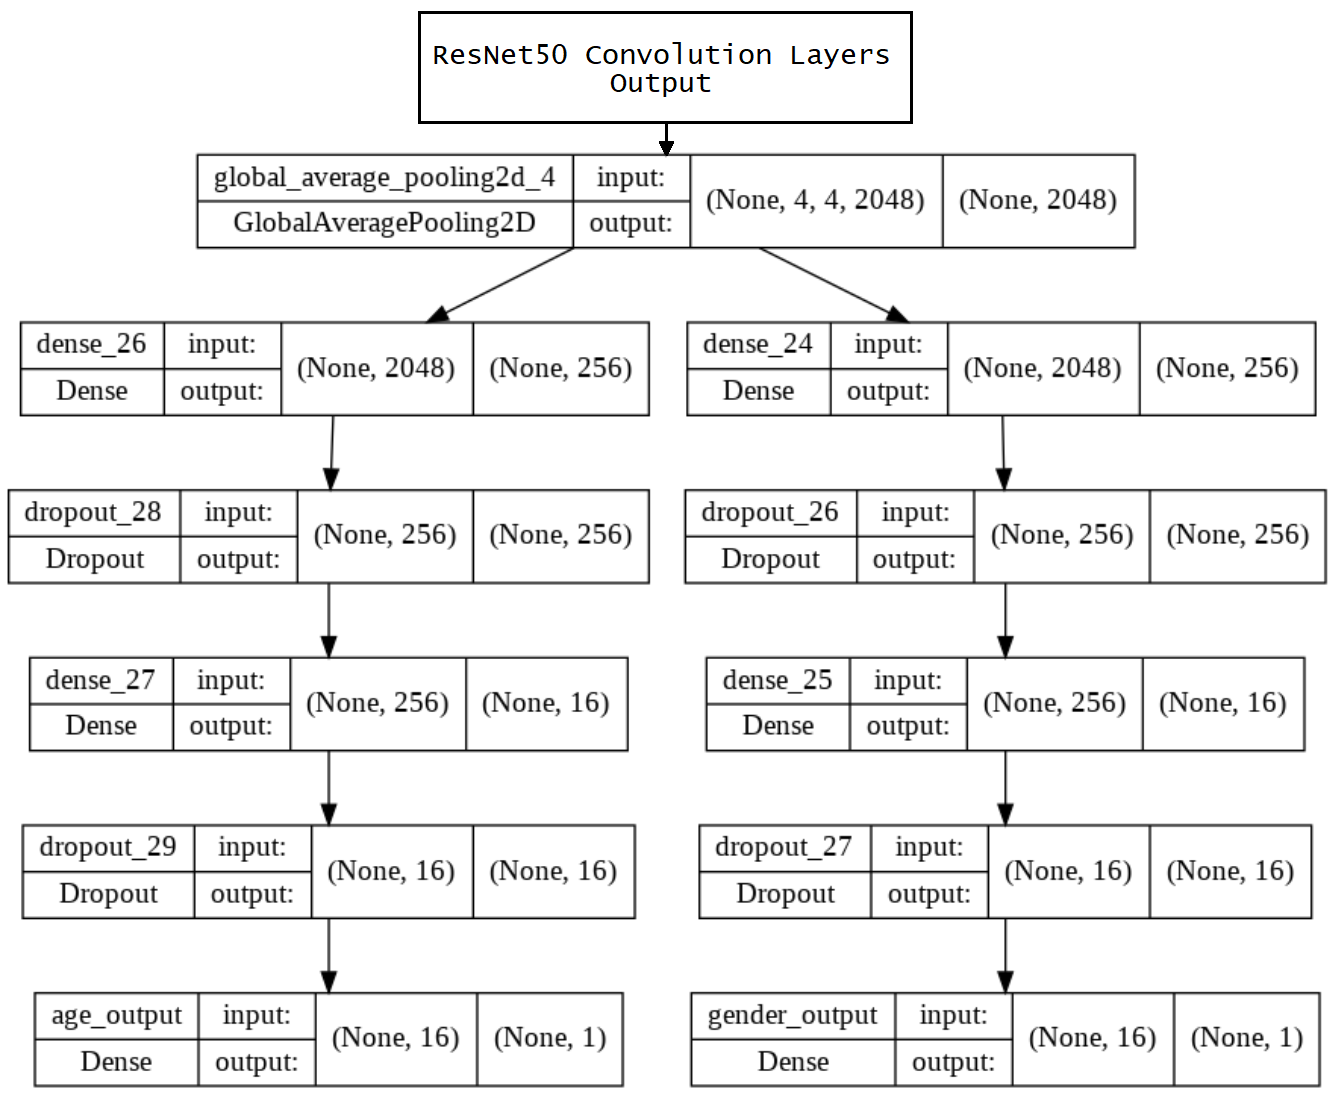
\includegraphics[height=0.5\textheight]{ModelBGraph_sample_simplified_dropouts_truncated.png}
\end{figure}
For our pre-trained model we used ResNet50 as our base. This is because it is a relatively fast, lightweight and high performing model (with respect to ImageNet top 5 rating).\\
We used weights trained on ImageNet as our initial weights.
These weights were not frozen in order to allow the model to learn features specific to age and gender prediction.\\
The output of this base model is fed into 2 branches (one for gender, the other for age).
Each performs an additional padded convolution, before being flattened and passed on towards their own FCN layers (with one output layer and 2 hidden layers).
All the FCN Dense layers made use of dropout and regularisation to reduce over-fitting.

\subsection{Training}
The pre-trained model was trained in the same manner as Model A, with the same losses, loss weights, and optimizer. 

To limit over-fitting a stop early callback was used to end training if the validation loss failed to improve over 5 consecutive epochs.

Hyper-Parameters were tuned in the same manner as for Model A.\\
Hyper-parameters tuned were:
\begin{enumerate}
    \item Initial Learning rate
    \item Flatten Vs Global Pooling: whether to flatten the 3D output from the final convolution layers
    \item Feature depth of final convolution layer 
    \item Number of Units for first FCN layer 
    \item Dropout rate
    \item Regularisation 
\end{enumerate}
Once tuning completed, we rebuilt and trained the model with the tuned hyper-params fixed.

\subsection{Performance}
Looking at \autoref{fig:ModelBPerformance} you can see Model B achieved an accuracy of 89\% on gender prediction and a mean squared error of 6.5 on age prediction. \\
\autoref{fig:ModelBPerformanceAge} shows very little over-fitting, with both lines sticking very close together with some minor spikes from the validation curve.\\
Unfortunately the gender accuracy shown in \autoref{fig:ModelBPerformanceAge} highlights a not insignificant amount of over-fitting, where validation accuracy always being at least 2\% more than the training accuracy, and starting to diverge from ~epoch 10.

The trace of the final epoch is below.
\begin{verbatim}
Epoch 25/50
125/125 [==============================] - 37s 295ms/step 
- loss: 137.7862 
- age_output_loss: 85.8010 
- gender_output_loss: 0.1336 
- age_output_mean_absolute_error: 6.6296 
- gender_output_binary_accuracy: 0.9495 
- val_loss: 148.9740 
- val_age_output_loss: 84.2459 
- val_gender_output_loss: 0.2754 
- val_age_output_mean_absolute_error: 6.4352 
- val_gender_output_binary_accuracy: 0.8952
\end{verbatim}

\begin{figure}[h!]
    \begin{subfigure}{\textwidth}
        \centering
        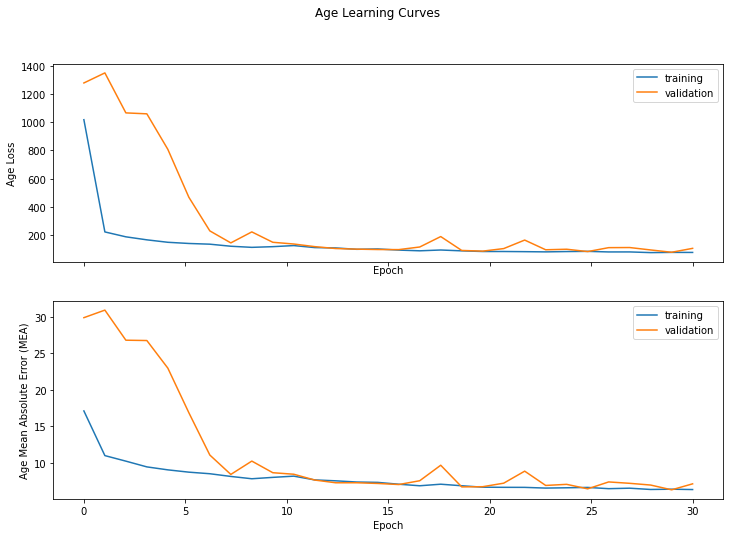
\includegraphics[height=0.45\textheight]{Model_B_AgeLearning_hp_tuned.png}
    \caption{\label{fig:ModelBPerformanceAge}The performance on age prediction for the pre-trained model.}
    \end{subfigure}
    \begin{subfigure}{\textwidth}
        \centering
        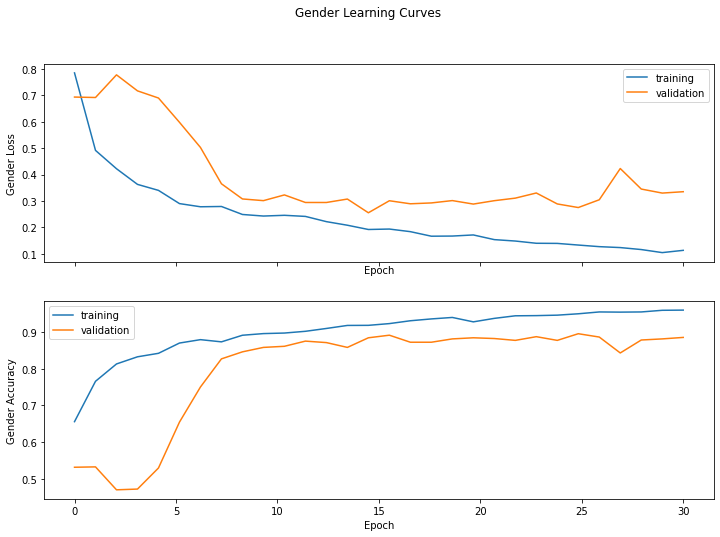
\includegraphics[height=0.45\textheight]{Model_B_GenderLearning_hp_tuned.png}
        \caption{\label{fig:ModelBPerformanceGender}The performance on gender prediction for the pre-trained model.}    
    \end{subfigure}
    \centering
    \caption{
        \label{fig:ModelBPerformance}Learning curves observed training Model B. \textit{Graphs show 30 epochs, however the weights are actually saved for epoch 25.}
        }
\end{figure}

